\documentclass[12pt]{article}
\usepackage{graphicx}
\usepackage{amsmath}
\usepackage{float}
\usepackage{array}

\title{Lab 4: Focusing Laser Beams with a Lens}
\author{Arnav Menon \\ School of Physics, Georgia Institute of Technology}
\date{February 14, 2025}

\begin{document}

\maketitle

\section{Introduction}
The purpose of this lab is to study the focusing of a Gaussian laser beam using a converging lens. By measuring the beam width as a function of distance near the focal point, we aim to determine the beam waist (\(w_0\)) and the Rayleigh length (\(z_R\)), which characterize the focus of the beam. This experiment is performed for two different initial beam diameters to observe how the focusing behavior changes with the initial beam size. The results are compared with theoretical predictions based on Gaussian beam optics, and the intensity of the focused beam is calculated to understand the effect of focusing on the beam's power density.

\section{Theory}
When a collimated Gaussian laser beam passes through a converging lens, it is focused to a point at a distance equal to the focal length (\(f\)) of the lens. The beam's transverse intensity profile is given by:
\[
I(r) = I_0 e^{-2r^2 / w^2},
\]
where \(I_0\) is the peak intensity, \(r\) is the radial distance from the beam center, and \(w\) is the beam width. The beam width varies along the propagation axis \(z\) as:
\[
w(z) = w_0 \sqrt{1 + \left(\frac{z}{z_R}\right)^2},
\]
where \(w_0\) is the beam waist (minimum width at the focus), and \(z_R\) is the Rayleigh length, given by:
\[
z_R = \frac{\pi w_0^2}{\lambda}.
\]
The Rayleigh length represents the depth of focus, i.e., the range over which the beam remains relatively focused. When a lens focuses a collimated beam, the minimum focus size (waist) is given by:
\[
w_0 = \frac{\lambda f}{\pi w_f},
\]
where \(w_f\) is the beam width at the lens, and \(\lambda\) is the wavelength of the laser.

\section{Near the Laser}
For the near case, the laser beam was focused using a 100 mm lens placed approximately 0.5 meters from the laser. The initial beam width (\(w_f\)) was measured to be 455.801 \(\mu\)m. The beam width was measured at various positions near the focus, and the data was fitted to the Gaussian beam equation to determine the beam waist and Rayleigh length.

\begin{figure}[H]
    \centering
    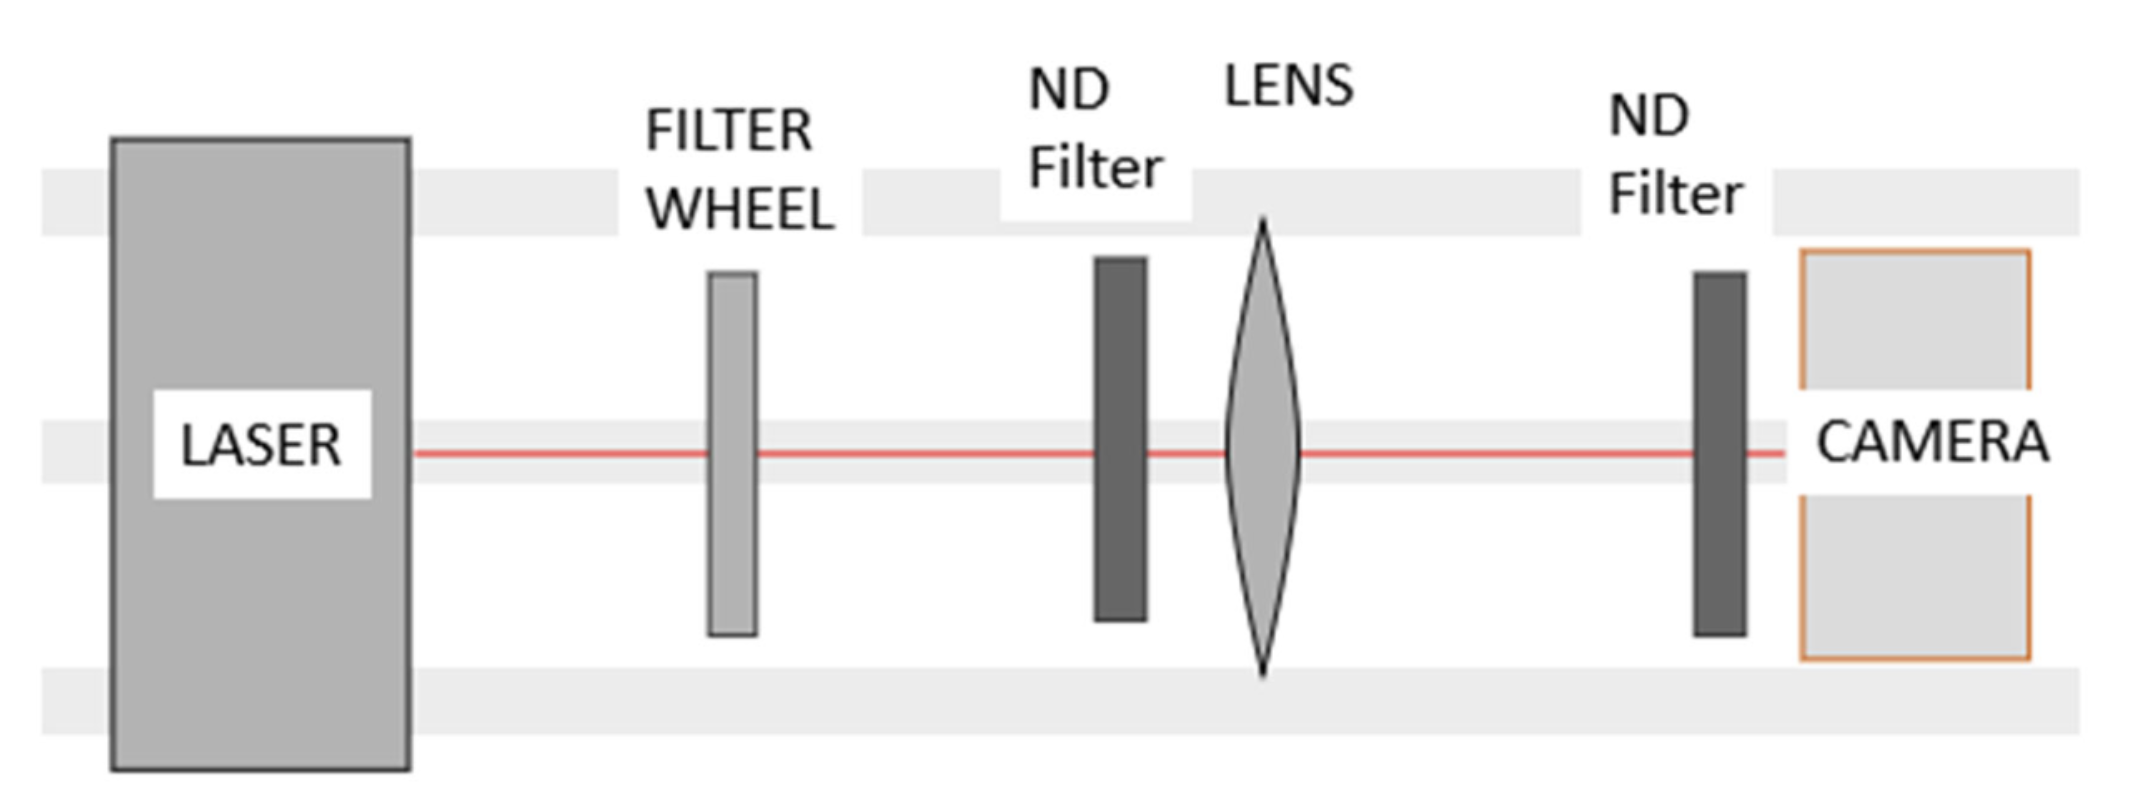
\includegraphics[width=1\linewidth]{Near_Diagram.png}
    \caption{Diagram of experimental setup for the near case.}
    \label{fig:near-setup}
\end{figure}

\begin{figure}[H]
    \centering
    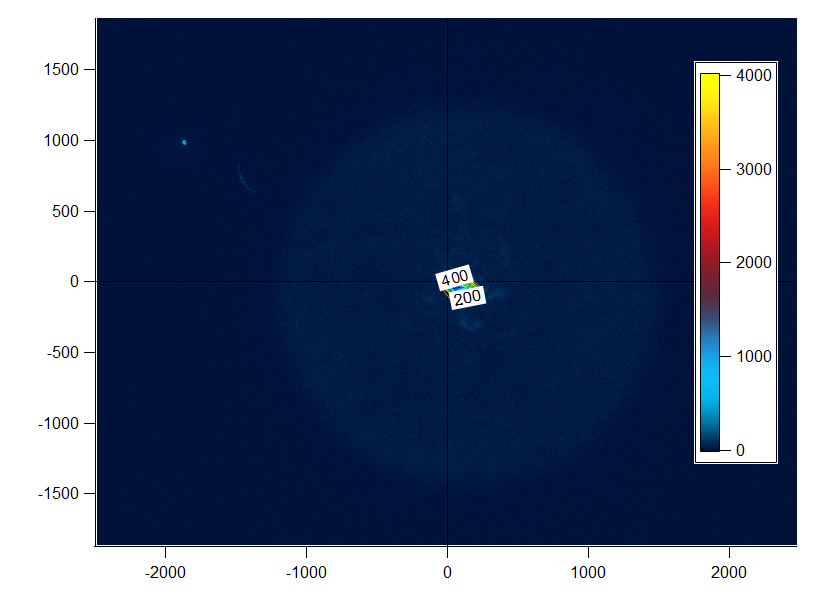
\includegraphics[width=1\linewidth]{Near_Focus.png}
    \caption{Near focus image of cross-section of the beam.}
    \label{fig:near-focus}
\end{figure}

The curve fitting process involved fitting the measured beam widths to the equation:
\[
w(z) = w_0 \sqrt{1 + \left(\frac{z - z_0}{z_R}\right)^2},
\]
where \(z_0\) is the offset of the origin. The fitted parameters were used to determine the beam waist and Rayleigh length.

\begin{figure}[H]
    \centering
    \includegraphics[width=1\linewidth]{Near_fit.png}
    \caption{Data taken near the laser (about 0.5 meters away) and the Gaussian fit to the data. The distance axis is shifted so that the focus of the beam lies at zero.}
    \label{fig:near-fit}
\end{figure}

\section{Far from the Laser}
For the far case, the laser beam was focused using the same 100 mm lens, but the lens was placed approximately 1.4 meters from the laser. The initial beam width (\(w_f\)) was measured to be 629.75 \(\mu\)m. The beam width was measured at various positions near the focus, and the data was fitted to the Gaussian beam equation to determine the beam waist and Rayleigh length.

\begin{figure}[H]
    \centering
    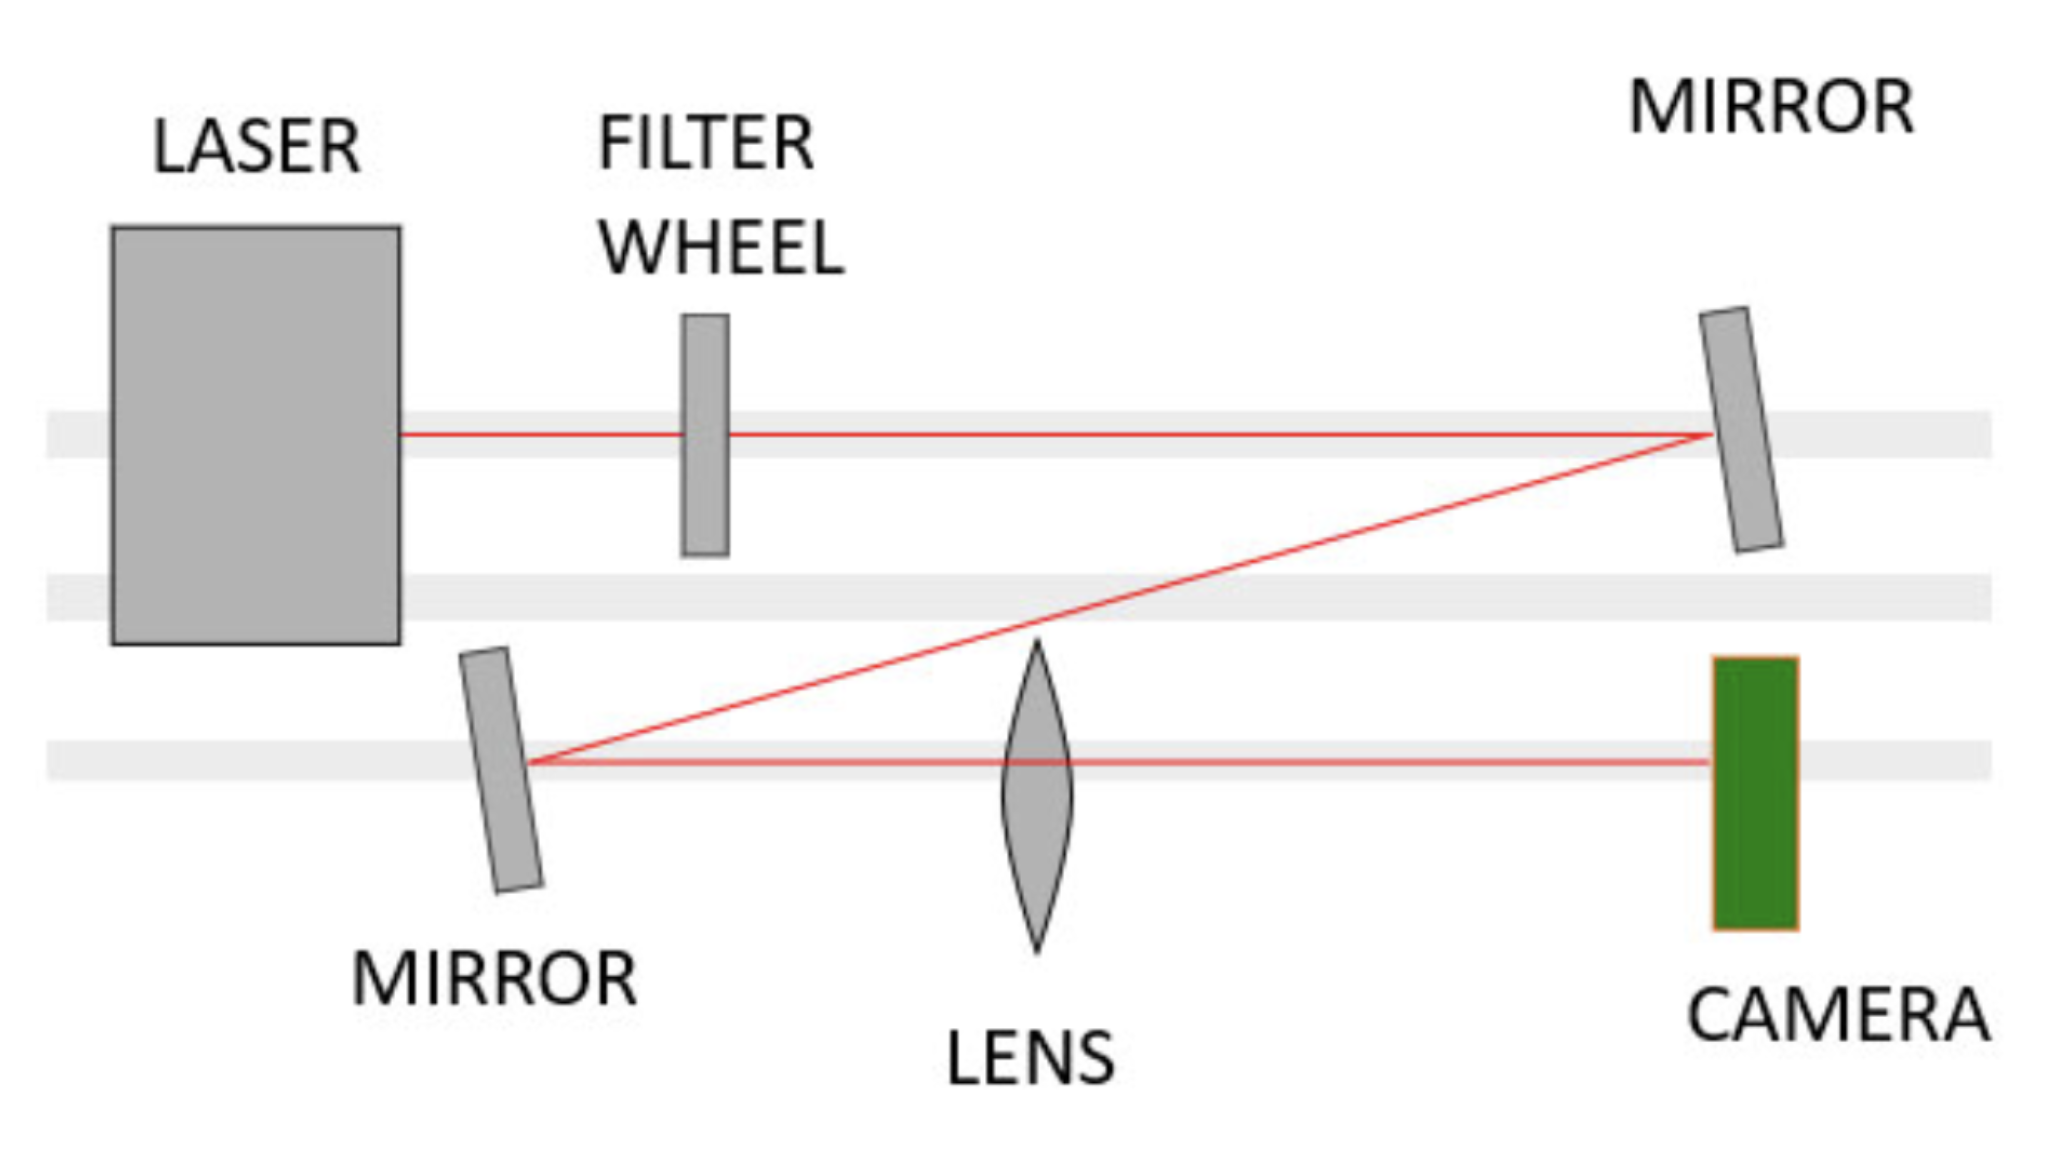
\includegraphics[width=1\linewidth]{Far_Diagram.png}
    \caption{Diagram of experimental setup for the far case.}
    \label{fig:far-setup}
\end{figure}

\begin{figure}[H]
    \centering
    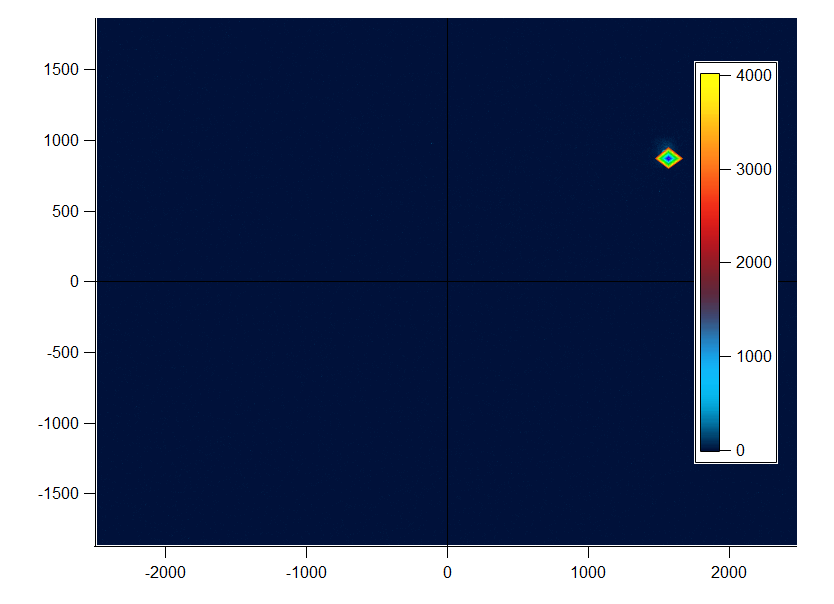
\includegraphics[width=1\linewidth]{Far_Focus.png}
    \caption{Far focus image of cross-section of the beam.}
    \label{fig:far-focus}
\end{figure}

The curve fitting process was similar to the near case, with the beam widths fitted to the Gaussian beam equation to determine the beam waist and Rayleigh length.

\begin{figure}[H]
    \centering
    \includegraphics[width=1\linewidth]{Far_fit.png}
    \caption{Data taken far from the laser (about 1.4 meters away) and the Gaussian fit to the data. The distance axis is shifted so that the focus of the beam lies at zero.}
    \label{fig:far-fit}
\end{figure}

\section{Discussion}
In the near case, the measured minimum beam waist was \(6.43 \times 10^{-5}\) meters, while the theoretically expected value was \(4.42 \times 10^{-5}\) meters. In the far case, the measured minimum beam waist was \(2.09 \times 10^{-5}\) meters, while the theoretically expected value was \(3.20 \times 10^{-5}\) meters. The discrepancies between the measured and theoretical values can be attributed to several factors:
\begin{itemize}
    \item Alignment errors: Small misalignments in the lens or beam path can lead to deviations from the ideal Gaussian focus.
    \item Beam quality: Real laser beams may not be perfectly Gaussian, leading to deviations from the theoretical predictions.
\end{itemize}

The far beam is focused more tightly than the near beam because the initial beam width is larger, leading to a smaller convergence angle and a tighter focus. This is consistent with the theoretical prediction that the beam waist is inversely proportional to the initial beam width.

Using the known power output of the laser (0.5 mW) and the measured beam widths, the intensities of the focused and unfocused beams were calculated. The results are summarized in the table below:

\begin{table}[H]
    \centering
    \begin{tabular}{|c|c|}
        \hline
        \textbf{Case} & \textbf{Intensity $(\text{mW}/\text{mm}^2)$} \\
        \hline
        Unfocused beam near the laser & 0.766 \\
        Focused beam near the laser & 38.494 \\
        Unfocused beam far from the laser & 0.401 \\
        Focused beam far from the laser & 364.357 \\
        \hline
    \end{tabular}
    \caption{Intensities of the unfocused and focused beams for the near and far cases.}
    \label{tab:intensities}
\end{table}

\section{Conclusion}
In this lab, we successfully focused a Gaussian laser beam using a converging lens and measured the beam waist and Rayleigh length for two different initial beam diameters. The experimental results were compared with theoretical predictions, and discrepancies were analyzed in terms of alignment errors, beam quality, and lens aberrations. The intensity of the focused beam was found to be significantly higher than that of the unfocused beam, demonstrating the effect of focusing on the beam's power density. This experiment provided valuable insights into the behavior of Gaussian beams and the practical challenges of focusing laser beams with lenses.

\end{document}


